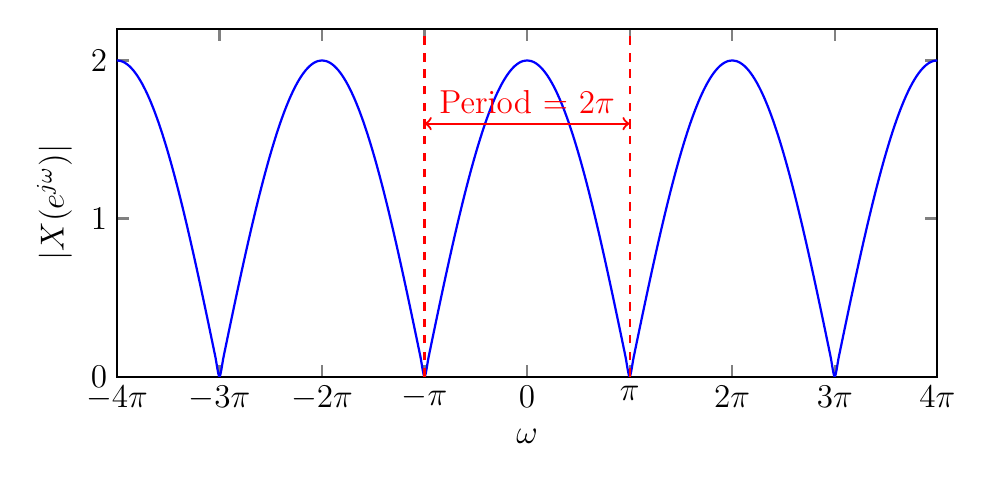
\begin{tikzpicture}
	\begin{axis}[
		width=12cm,
		height=6cm,
		xlabel={$\omega$},
		ylabel={$|X(e^{j\omega})|$},
		xmin=-4*pi, xmax=4*pi,
		ymin=0, ymax=2.2,
		xtick={-4*pi, -3*pi, -2*pi, -pi, 0, pi, 2*pi, 3*pi, 4*pi},
		xticklabels={$-4\pi$, $-3\pi$, $-2\pi$, $-\pi$, $0$, $\pi$, $2\pi$, $3\pi$, $4\pi$},
		ytick={0, 1, 2},
		domain=-4*pi:4*pi,
		samples=201,
		smooth,
		axis line style={thick},
		tick style={thick},
		label style={font=\large},
		tick label style={font=\large},
		every axis plot/.append style={thick},
		]
		% Plot the magnitude spectrum as 2*|cos(ω/2)|
		\addplot[blue] {2*abs(cos(deg(x/2)))};
		
		% Vertical dashed periodicity lines at -2π and 2π
		\addplot[red, dashed] coordinates {(-pi, 0) (-pi, 2.2)};
		\addplot[red, dashed] coordinates {(pi, 0) (pi, 2.2)};
		
		% Periodicity arrow with label above the curve
		% The non-breaking space between the coordinate and the 'node' command was replaced
		% with a regular space.
		\draw[<->, thick, red] (axis cs: -pi, 1.6) -- (axis cs: pi, 1.6)
		node[midway, above, font=\large] {Period = $2\pi$};
	\end{axis}
\end{tikzpicture}